\documentclass[11pt,a4paper]{article}

% Packages for formatting and graphics
\usepackage[utf8]{inputenc}
\usepackage{geometry}
\usepackage{graphicx}
\usepackage{listings}
\usepackage{xcolor}

% Page geometry
\geometry{margin=2.5cm}

% R code styling
\definecolor{codegreen}{rgb}{0,0.6,0}
\definecolor{codegray}{rgb}{0.5,0.5,0.5}
\definecolor{codepurple}{rgb}{0.58,0,0.82}
\definecolor{backcolour}{rgb}{0.95,0.95,0.92}

\lstdefinestyle{rstyle}{
    backgroundcolor=\color{backcolour},   
    commentstyle=\color{codegreen},
    keywordstyle=\color{magenta},
    numberstyle=\tiny\color{codegray},
    stringstyle=\color{codepurple},
    basicstyle=\ttfamily\footnotesize,
    breakatwhitespace=false,         
    breaklines=true,                 
    captionpos=b,                    
    keepspaces=true,                 
    numbers=none,                    
    showspaces=false,                
    showstringspaces=false,
    showtabs=false,                  
    tabsize=2,
    frame=single,
    rulecolor=\color{blue!30!black}
}

\lstset{style=rstyle}

\begin{document}

\begin{lstlisting}[language=R]
library(ggplot2)

# Set working directory and read data
setwd("/home/vicente/projeto-pe-2024-2025/Exercicio3")
dados_clima_raw <- read.csv("clima.csv")

# Convert datetime and filter for November 2014
dados_clima_raw$datetime <- as.POSIXct(dados_clima_raw$Data)
dados_clima_raw$year <- as.numeric(format(dados_clima_raw$datetime, "%Y"))
dados_clima_raw$month <- as.numeric(format(dados_clima_raw$datetime, "%m"))
dados_clima_raw$date <- as.Date(dados_clima_raw$datetime)

# Filter for November 2014
dados_clima <- dados_clima_raw[dados_clima_raw$year == 2014 & dados_clima_raw$month == 11, ]

# Calculate daily median pressure
daily_medians <- aggregate(Pressao ~ date, data = dados_clima, FUN = median, na.rm = TRUE)
names(daily_medians)[2] <- "mediana_pressao_diaria"

# Merge back with original data
dados_clima <- merge(dados_clima, daily_medians, by = "date")

# Create and save plot
plot <- ggplot(dados_clima, aes(x = datetime)) +
  geom_line(aes(y = Pressao, color = "Pressao Horaria"), alpha = 0.7) +
  geom_line(aes(y = mediana_pressao_diaria, color = "Mediana Diaria"), linewidth = 1) +
  labs(title = "Variacao da Pressao Atmosferica em Novembro de 2014",
       x = "Data e Hora", y = "Pressao (hPa)", color = "Legenda") +
  scale_x_datetime(date_breaks = "3 days", date_labels = "%d/%m") +
  scale_color_manual(values = c("Pressao Horaria" = "deepskyblue", "Mediana Diaria" = "red4")) +
  theme_minimal() +
  theme(axis.text.x = element_text(angle = 45, hjust = 1), legend.position = "top")
\end{lstlisting}

\begin{figure}[htbp]
    \centering
    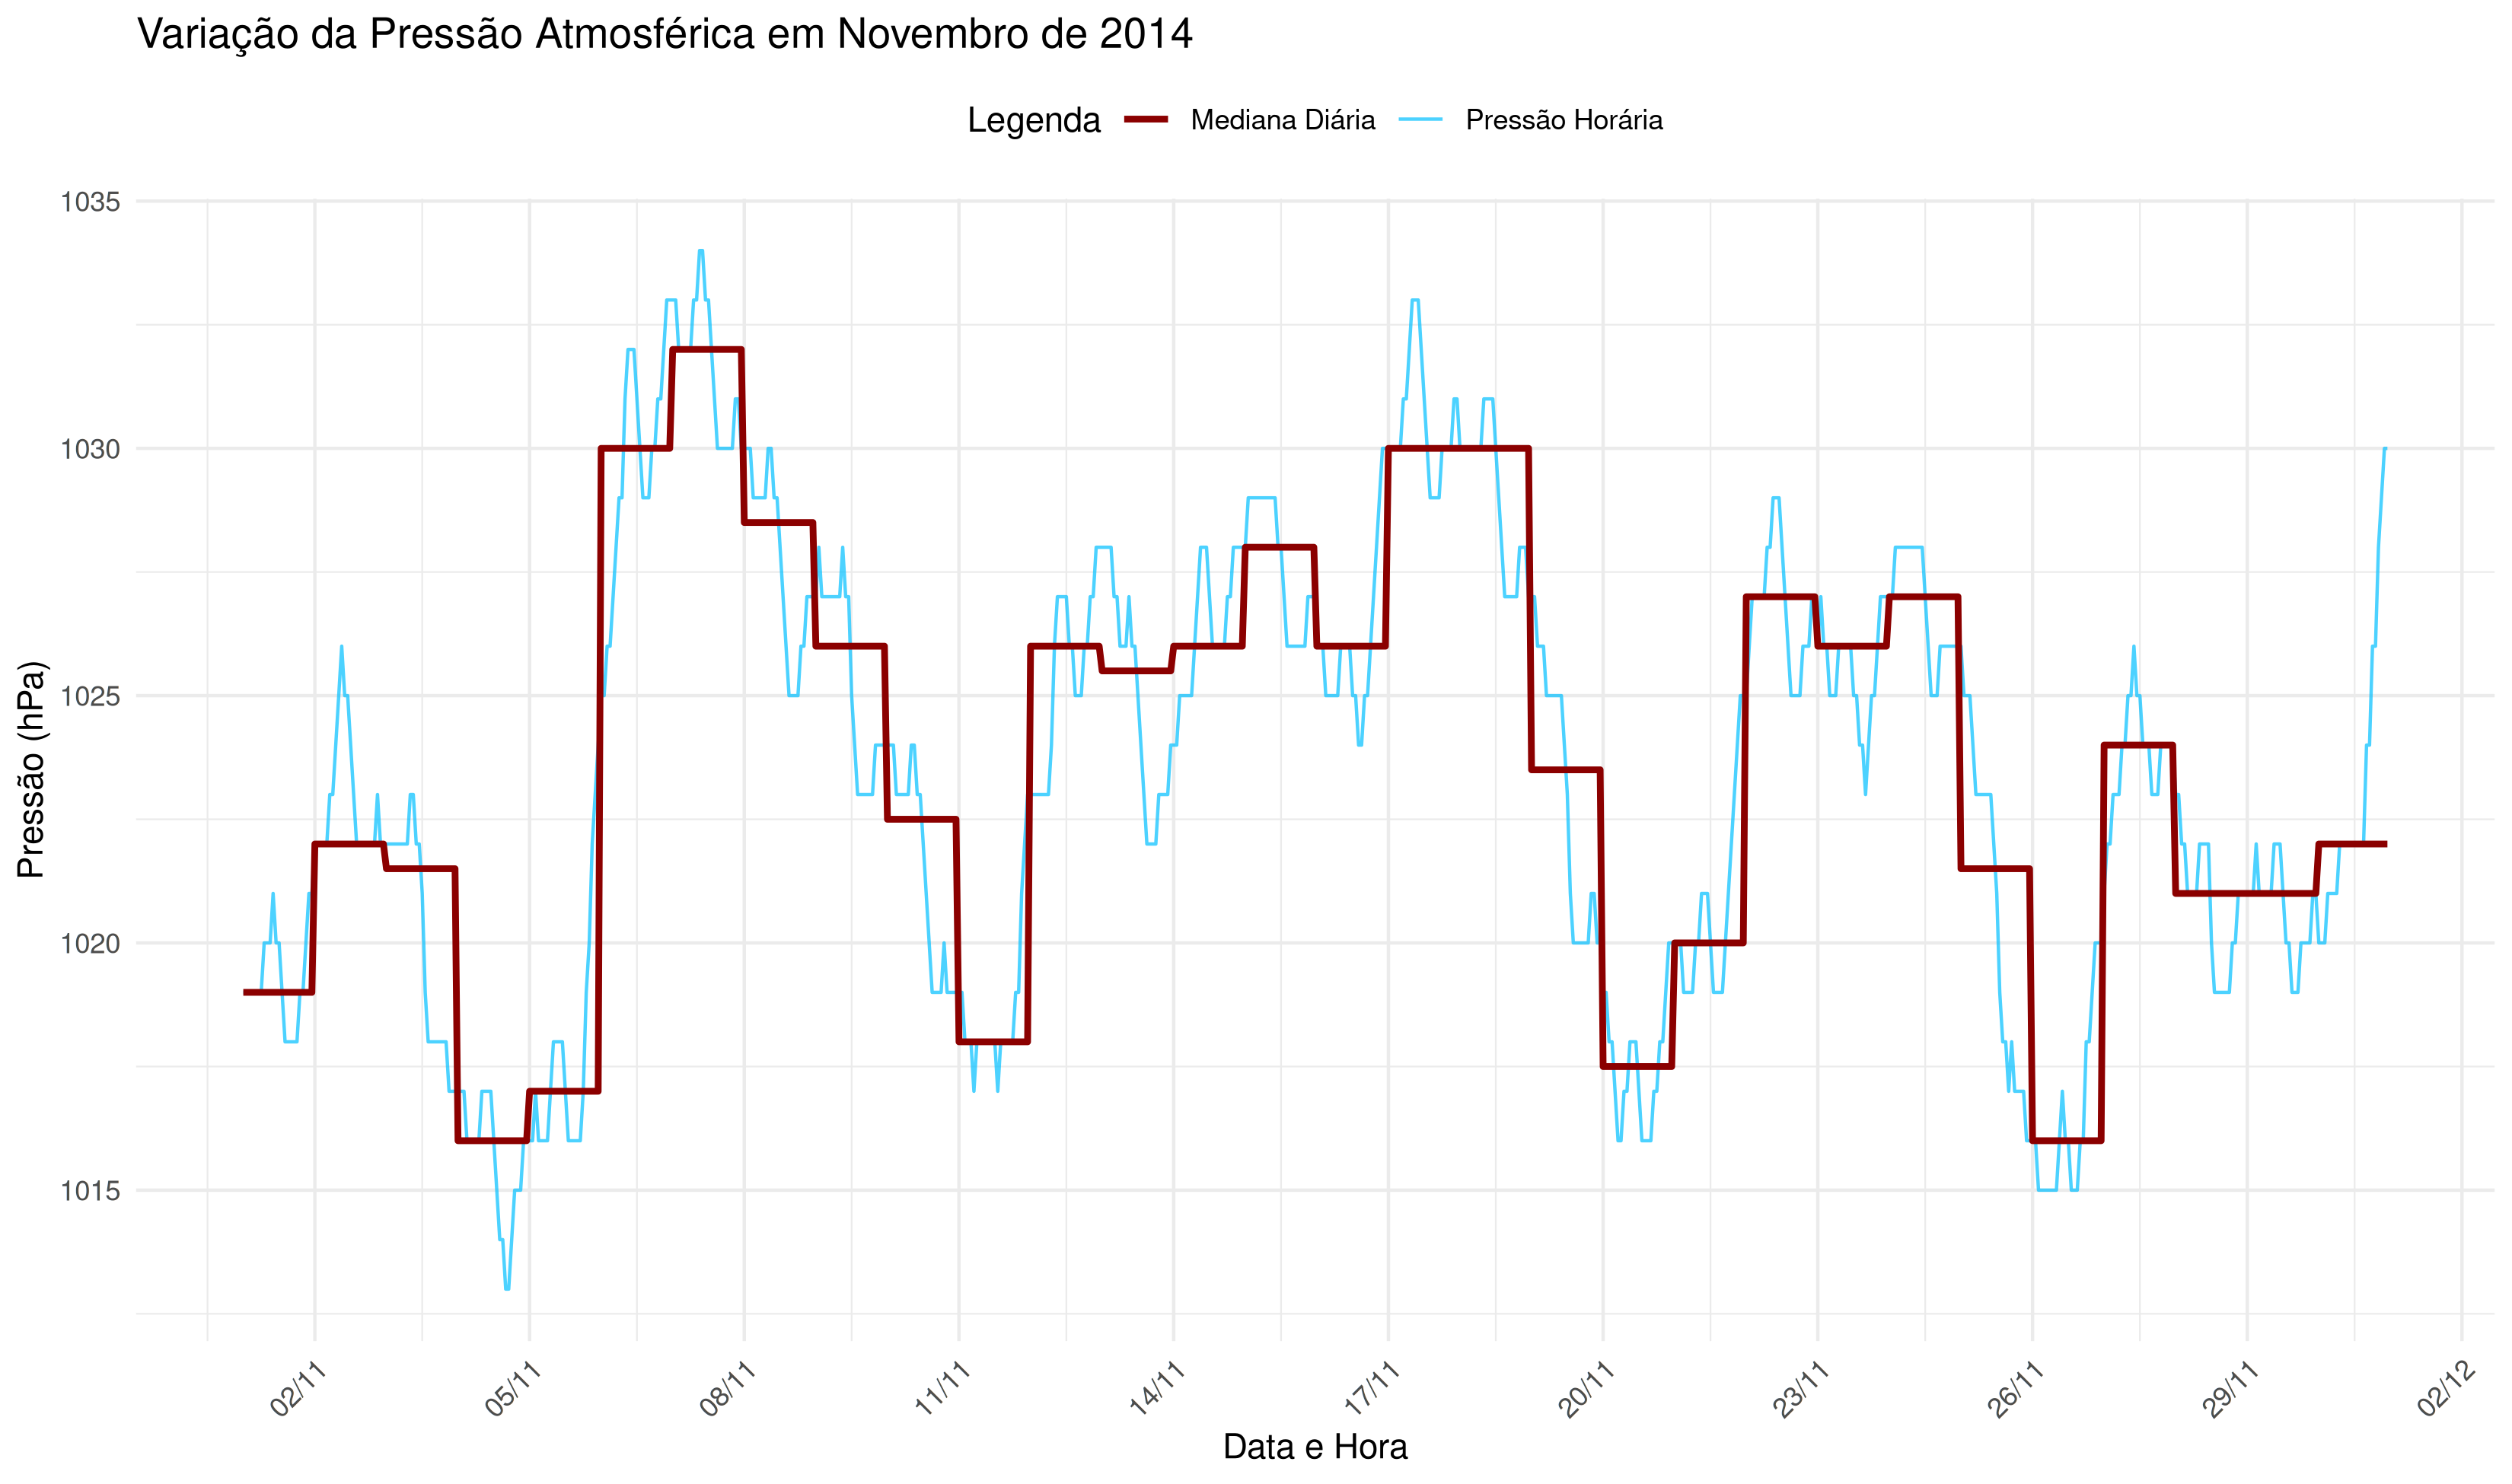
\includegraphics[width=0.9\textwidth]{clima_pressao_nov2014.png}
\end{figure}

\end{document}
